\chapter{}
Tuesday morning was busy. We got up early, ate a quick breakfast, and I left Monique at
home in her wheelchair with her laptop while I dropped her truck off at the body shop. I caught
a cab ride home, stopping at a leather shop along the way. Once I was home, we headed out to do
some shopping. Getting her into my truck was even more difficult than her SUV, but I knew that
this was the last day I'd be struggling with it. We had to go several places, but we finally
acquired enough clothing that would work with her cast, or be easily modified to work with it.

It was nearly noon when we'd finished, and we stopped for a quick bite at the local coffee
shop before heading home. The weather was nice, so we sat outside at a table, and enjoyed our
lunch almost as much as we enjoyed the attention that Monique drew. The best was from a young
boy, no more than three or four, who was walking into the coffee shop with his mother: ``Mommy-
that lady gots a big boo-boo!'' he said. His mother looked a bit embarrassed, but Monique just
smiled at them.

On the way home, we noticed a tailoring/dry cleaning establishment with a sign in the window
stating that they had one day service on alterations. I pointed it out to Monique, and she
agreed that it would probably be a lot easier than trying to find a decent position for her to
work on the changes herself. The ladies working there were understandably taken aback when they
first saw Monique, but the seamstress worked with Monique, giving suggestions as they talked
about the modifications to be made.

Back home, Monique wanted to do some work for her classes. I took her to the hospital room
and laid her on the bed. While she studied, I read a magazine. Even though she'd been in the
cast for a few days, I still found myself sneaking glances at her. I was still amazed to be with
such a wonderful, beautiful woman. She loved being in the cast. She'd not only chosen to wear
the cast, but had even schemed to wear it for an extended period of time. Truly an amazing woman
and I was a very lucky man to have found her.

\begin{thought}
Monique was productive, looking over the syllabi for her classes, and doing some of the
initial reading, but occasionally, her thoughts would drift. She noticed Quinn looking at her a
few times, and she could easily drift into thinking about how much her life had changed in the
past few months, and how much she loved it. And occasionally, her thoughts tried drifting to her
current adventure: She was now over four days into wearing this cast. It was as big a cast as
she'd ever worn, and this was twice as long as she'd ever worn a big cast. She was moving into
new territory, and it was fascinating for her. She'd experienced some cramping early on, as she
did with every cast. Today was different, though. There had been no cramping at all today. It
had become as if her legs and hips were somewhat disconnected from her consciousness. She could
see them, captured in the solid plaster, and if she tried to flex them, she could feel the
restraint holding them still. But, they'd become almost like her heart or lungs- still a part of
her, and a part she could feel if she tried, but a part hidden under her new outer ``skin.''
This
was an entirely new aspect to wearing casts for her. Before, the cast had been something she'd
worn, and loved wearing. Now, it was almost becoming a part of her.
\end{thought}

At about 4:30, the body shop called to say that Monique's Expedition was ready. I called a
taxi, and when it arrived, I kissed her and excused myself with a promise to be back soon with
our new ``toy.''

When I got to the body shop, I examined the work that had been done, and was very pleased.
It was done exactly how I'd envisioned it, and the workmanship appeared to be superb. I paid the
bill, and hurried home, anxious to try out the new equipment.

Monique was reading, but she occasionally found her thought drifting to wonder about what
sort of contraption Quinn had dreamed up. She was excited to try it out. From what Quinn had
described, it should make loading and unloading a seriously immobilized person an easy task. By
having these modifications made, Quinn was showing her that he had plans to need help lifting
her in and out of the vehicle in the future, too. This wasn't some passing fancy for him, and
that suited her just fine.

When I walked into the hospital room, Monique greeted me with a kiss, followed quickly by
``Let's go see what you've done to my truck!''

I moved her to the wheelchair, and took her outside to see what I'd done. I opened both
doors on the passenger side so that she could see the lift completely before we tried it out.

``Here it is,'' I told her.

What Monique saw was a round upright bolted to a plate on the floor just behind the front
seats. It extended almost to the top of the passenger compartment, then had a square tube
fastened to it at a ninety degree angle, which went toward the driver's side. The square tube
had a small black box at the end that looked like it might be a motor.

``OK. How does it work?'' she asked.

``I was hoping you'd ask that,'' I said with a smile. As you see it, it's locked into the
travelling position. When locked, it will not move around. But, if you pull this pin out (I
removed a pin near where the round upright mounted to the floor), the whole assembly swivels. It
is on a set of two bearings, so it swivels easily, even with a load.'' I swung the arm around
toward the open passenger door.

``So that's what I am. A load. Hmm'' she scowled. Of course, the scowl was done playfully.
Her great sense of humor was one of the things I loved about her. Of course, I had to give her a
little grief right back.

``In that cast, you ARE a load. A beautiful load, but a load, nonetheless.''

I went on. ``With the crane swung around, we remove one more pin here on the arm.'' I took
out the pin that locked the arm extension. ``With that, I can extend the arm quite a bit. I
don't
even have to have you right next to the truck to lift you.'' I rolled her slightly forward,
until
she was even with the front door opening. ``The arm telescopes out on linear bearings, for ease
of movement.''

``You put a lot of thought into this,'' she said.

``I want something that will serve us for a long time, and serve us well. I'm hoping we
continue to need it from time to time.''

``If I have any say in it, we will,'' Monique answered.

``Now, with the end of the arm directly over you, I lower the cable.'' There was a small
control box attached to the winch by a 3 foot cable. I stood next to Monique and pushed the
button to lower the cable. When the hook was nearly touching her midsection, I stopped.

``And now, to get you hooked up.'' I said. From the passenger front floorboard, I got the
harness that the leather shop had made for me. It had three sturdy belts with rings on them. I
fastened the large belt of the three around her waist and each of the smaller ones around her
legs at the thigh. Next was the connector strap. It attached to the belt at her waist, and the
straps on each leg. It had rings at several points, so I could use the one that best balanced
her for the lift. I took an educated guess, and attached the hook to one of the rings.

``Are you ready to see this in action?'' I asked.

``You bet!'' she answered.

I pressed the button on the control to lift, and I noticed her lower body rising, but her
shoulders were still on the back of the chair. I lowered her back and tried a different ring,
closer to her head.

\begin{thought}
Feeling herself being lifted was very odd to Monique. As she rose off of the chair, she
took hold of the connecting strap to keep her upper body in line. Even so, it still almost felt
as if she were watching some inanimate object else being lifted. She had no sensation of the
straps around her waist and legs. Her lower body was so used to the cast; it was almost as
though it were not attached.

Quinn lifted her until her waist was almost touching the arm. He then turned her so that
her head went in first and gently pushed her. The arm telescoped back in easily and smoothly,
and it turned easily, too. Quinn had to do a bit of swiveling to get her situated inside the
truck. When she was over the seat, he pushed the other button and she lowered gently to the
seat. It was comfortable, it was smooth, and it was obviously easy for Quinn. With this, he
could easily load her in the truck, no matter what sort of cast or casts she was wearing. Even a
full body cast.

Even a full body cast. Hmm.
\end{thought}

Once Monique was lowered into place, I removed the hook from its ring on the harness and
retracted the cable. With that done, I pushed the arm back in and set the locking pin. I
finished by swinging the arm around to the driver's side and set the pin that locked the
rotation.

``That looked easy.'' She said.

``It WAS easy,'' I replied.

``So- I'm all loaded up. Are we going to go anywhere?''

I suggested dinner, and we headed to a local restaurant. It was odd- I'd been several
places with her in casts before, but this was the first time we'd done it so close to home. It
was definitely a new experience. She saw a couple of people she knew from school, and they of
course were shocked to hear of her ``injuries'' from the building collapse during the storm.

Things over the next few days smoothed out a bit over the first few days in the cast. We
were getting used to dealing with living life with her immobilized. Friday morning, I stood her
up at the sink in the bathroom so she could get ready for school. Realizing that this would be
her last morning in this cast, I decided to do one last drawing of her wearing it. I sketched
her as she stood at the sink.

When she was finished, I helped her dress, and we headed out for her last day in the
plaster double hip spica.

\newpage
\begin{center}
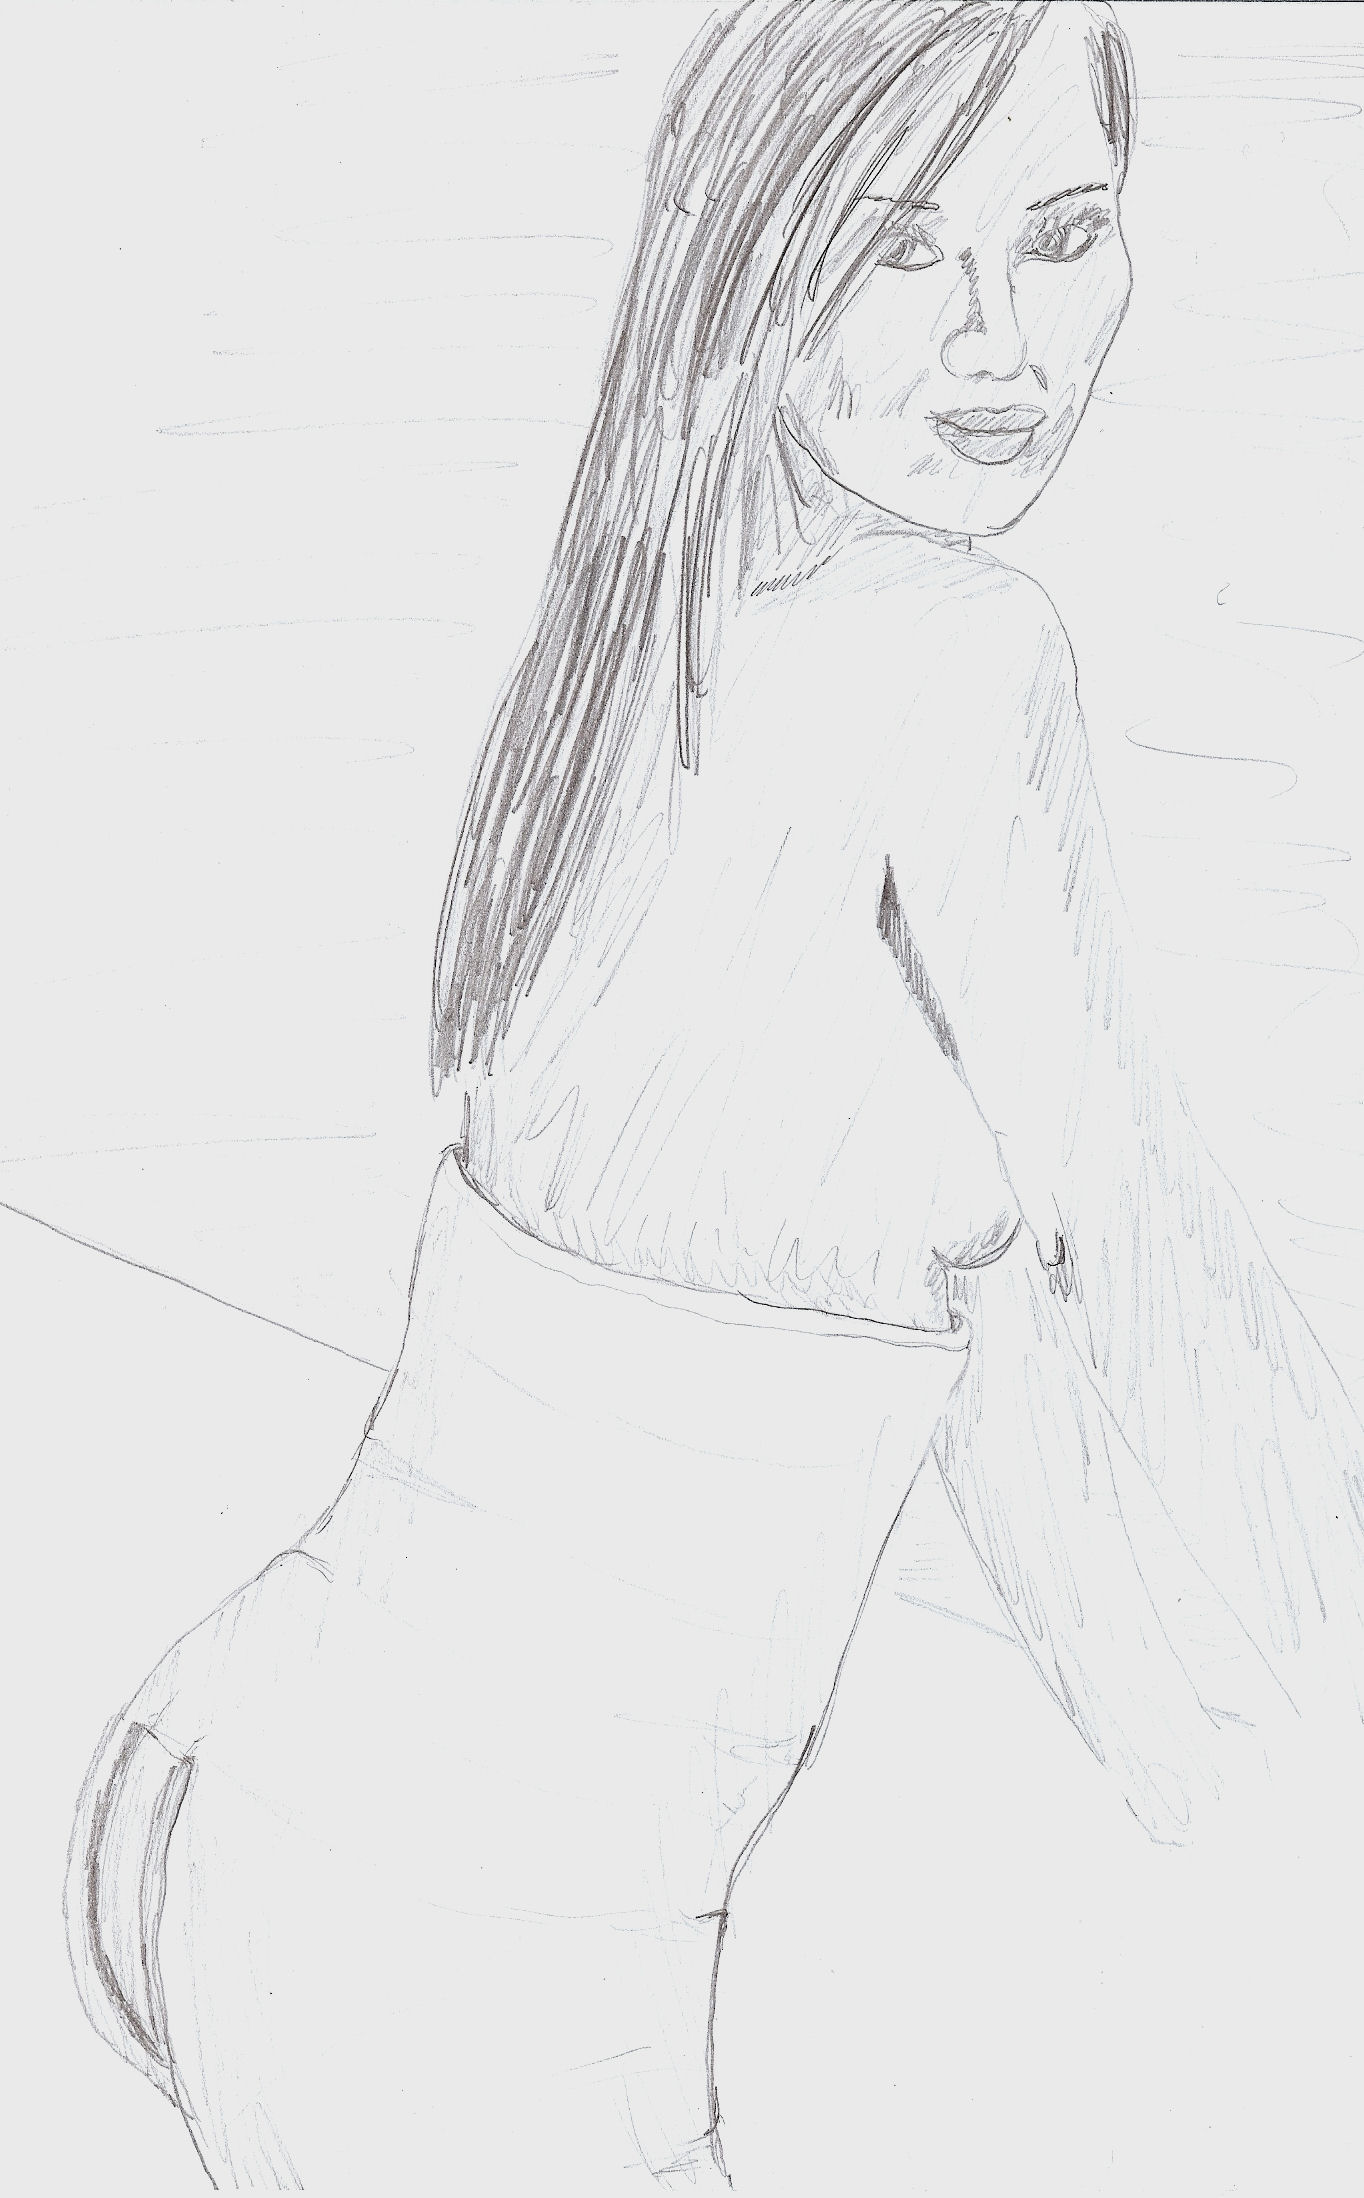
\includegraphics[height=\textheight]{images/kicks46.jpg}
\end{center}
